\documentclass[a4paper,13pt, margin=0.9in]{article}
\usepackage{graphicx} 
\usepackage{sectsty}
\usepackage{mathptmx}


\linespread{1.5}

\begin{document}

\begin{titlepage}
    \centering
    {\bfseries\Large
        NEWAR OF NEPAL\\
        \vskip1cm 
  
    
    } 
    A Brief Ethniographic Report submitted to Paschimanchal Secondary School for fulfillment of Practical Requirement of Annual Board Examination of Grade XII (Humanities) taken by NEB Nepal   
    \vskip1cm 
    
    
    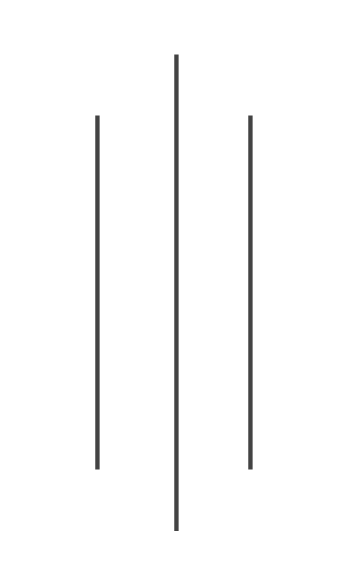
\includegraphics[width=3cm]{sample.png}
    \vskip1cm 
   
    \textbf{By:}
   
     Bishal Giri\\
     Class Roll No. 19 \\
     Class: XII (Humanities)
    
     \vskip0.5cm 
     
     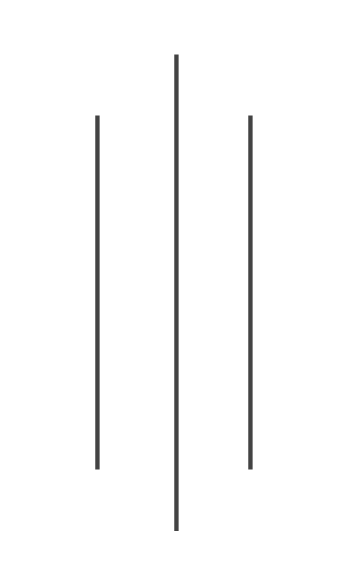
\includegraphics[width=3cm]{sample.png}
     
     \vskip0.5cm 
     
     Paschimanchal Secondary School \\
     Pokhara-4, Gairapatan \\
     2076
\end{titlepage}

\begin{flushleft}
\section*{ACKNOWLEDGEMENT}
I am highly indebted to my teacher Mr. Amrit Kumar Bhandari for his guidance and constant supervision as well as for providing necessary information regarding the project and also for his support on completing the project. I would like to express my gratitude towards my parents for their kind co-operation completion of this work.
\vskip0.5cm 
	
	
	I would like to express my special gratitude and thanks to those person of Newari community for giving me such an attention and their precious time.
	\vskip0.5cm 
	
	My thanks and appreciations also go to my classmate in developing the project and to the people who have project  and to the people who have willingly helped me out with their abilites.
	\vskip0.5cm 
	
	Thank you 
	
	



\begin{flushright}
		Bishal Giri
\end{flushright}


\newpage
\tableofcontents

\newpage

\section{ORIGIN AND SETTLEMENTS}

	The Newars are regarded as the original inhabitants of the Kathmandu Valley, but their origins are shrouded in mystery. They speak a Tibeto-Burmese language, which indicates they originated in the east, but their physical features range from distinctively Mongoloid, again suggesting to east, to Indo-Aryan, which of course points to India.
	\vskip0.5cm 

In balance, it seems most like that the Kathmandu valley has long been a cultural and racial melting pot, with people coming from both east and west. This fusion has resulted in the unique Newar culture that is responsible for the valley's superb art and architecture.
\vskip0.5cm 

The Newar golden age peaked in the 17th century when the valley consisted of small city-states, and Nepal was a vitally important trading link between Tibet and the north Indian plains. the valley's visible history is inextricably entangled with the Malla kings. It was during their reign, particularly in the 1600's and 1700's, that many of the valley's finest temples and palaces were built. Competition between the cities was intense and an architectural innovation in one place, such as the erection of a column bearing a statue of the ruling king, would inevitably be copied in the other cities.
\vskip0.5cm 

Sorting out who built what and when is considerably complicated by the fact that at any one time there was not just one Malla king. Each of the three city-states in the valley – Kathmandu, Patan and Bhaktapur – had its own.
\vskip0.5cm 

The unification of Nepal in 1768 by Gorkha's king Prithvi Narayan Shah signaled the end of the Kathmandu Valley's fragmentation. Nepali, an Indo-European language spoken by the Khas of western Nepal. replaced Nepalbhasa as the country's language of administration.

\newpage
\section{POPULATION DISTRIBUTION}
	
\begin{table}[htb]
\centering
\begin{tabular}{lllll}
\cline{1-3}

\multicolumn{1}{|l|}{\textbf{Ethnicity}} & \multicolumn{1}{l|}{\textbf{Population}} & \multicolumn{1}{l|}{\textbf{Total of Whole Population}} &  &  \\ \cline{1-3} 
\multicolumn{1}{|l|}{Newar}     & \multicolumn{1}{l|}{1,321,933}  & \multicolumn{1}{l|}{5\%}   &  &  \\ \cline{1-3} 
\end{tabular}
\end{table}

The given data is according to the Nepal's census, 2011 AD .


\newpage
\section{MAIN FEATURES OF SOCIO-CULTURAL LIFE}
\subsection{LANGUAGE}


"Newari" is vulgar term for the true name "Nepalbhasa" or "Nepalese" \\
- Dharmaditya Dharmacharya \\
(in a letter to Silvan Levi) \\

The Newars speak Nepal Bhasha, a Himalayan language of Tibeto-Burman branch of the Sino-Tibetan group. It has been incorrectly called by the term 'Newari' by westerners and non-Newars of Nepal. From the very beginning of history of Nepal it has been known as Nepal Bhasha. According to the research findings on this language it is proved that Nepal Bhasha shares the feature of Kirant and Tibetan dialects of Northen Himalayas. The colloquial term used by native speakers is Newaah Bhaaye. It consists of five major dialects and several sub-dialects spoken by Newars living throughout the country. \\

\subsubsection{Literature Extant}
Historical evidence indicates that many Nepal Bhasa words are found in Lichhivi inscriptions. Hence it has been assumed that the writings on this language was resumed from the early Malla period (9th Century) and it was adopted as the public language of Nepal. In the manuscript of 'Nidan' (901 A.D.) the date has been written in Nepal Bhasa- (Kwoyeya pwalam mikhaya pwalam sambat nepalaya thuli). The concluding line of 'Tathagat Guhyak' manuscript (1104 A.D.) shows Sidhayeka juro (here it ends). The Guthi documents (1114 A.D.) found in Rudravarna Mahavihar in Lalitpur, also indicates a long description written in Nepalbhasa Hence, from the very beginning of 12th century, Nepal Bhasa was used as independent language of expression. The stone inscriptions found in the courtyard of Vajrayogini Temple of Sankhu (dated 1173 A.D) and copper inscription found in Kasthamandap (dated 1374 A.D.) are the oldest monuments in Nepal Bhasa. \\

The oldest book (manuscript) in Nepalbhasa found till now is 'Guhya Kali Puja Bidhi' (1280 AD). Before it was found, 'Haramekhala' (1374 A.D.), a medicinal book translated from Prakrit language book written by Bengal Poet Madhuk was considered as the oldest nepalbhasa book. The other books found in that period are Nyayashastra (1380 A.D.), Putrapautradibodhini (1381 A.D.), Amarakosh (1386 A.D.) etc. The Gopalraj Vanshavali of 947A.D. (a chronicle) is the first original Nepalbhasa book, from which first sixteen pages have been still missing and pages 17 to 30 (A) uses the Sanskrit language while Nepal Bhasha is used in pages 30(B) to 63. \\

Dashaphala (1399A.D.), Bhasajyotis (1422 A.D.), Sumatikarana (1512 A.D.) and others can be mentioned in astrological book written in Nepalbhasa. 'Dashakarma Paddati' (1498 A.D.) is the oldest book on rituals written in Nepalbhasa. After 'Bhagwat Puran' (1505 A.D.), creative literature in Nepalbhasa starts from 'Tantrakhyan' (1518 A.D.).\\

\subsubsection{Creative Literature at a Glance}
First Story Book - Tantrakhyan (1518 A.D.)\\
First Song - Walangata Simule Swambaraya (In reign of Pranmol malla, 1523-1550 A.D.)\\
First One-act Play - Ekadashi Brata (1633A.D.) by Sidhhinarasingha Malla\\
First Drama - Mooldev Shashidev by Jagat Prakash Malla (1645-1673 A.D)\\


\newpage

	\subsection{RELIGION}
	Ask a Newar whether he's Hindu or Buddhist, the saying goes and he'll answer "yes" : after fifteen centuries of continuous exposure to both faiths, the Newars of the Kathmandu Valley have concocted a unique synthesis of the two. To religious scholars, the Newar religion is as exciting as a biologist's missing link, for some believe that it provides a picture of the way Mahayana and Vajrayana Buddhism functioned historically in India.\\

Until only the past two centuries, the Newars held fast to original monastic form of tantric Buddhism – as the bahal of Kathmandu and Patan still bear witness – while their rulers pursued the Hindu tantric path. However, the Kathmandu Valley has become progressively "Hinduized" since the unification of Nepal in the eighteenth century: the monasteries have largely disappeared, their monks have married, and the title of Vajracharya (Buddhist Priest) has become a hereditary caste like that of the Bahun (Brahman) priests. Today, Newar Buddhists are perhaps the only Buddhist culture that no longer maintains active communities of monks or nuns. Although the acceptance of caste and decline of monasticism have shifted the balance in favor of Hinduism, at the popular level the synthesis remains as well bonded as ever.\\

When Newars refer to themselves as Buddha Margi (Buddhist) or Shiva Margi (Hindu), they often do so only to indicate that they employ a Vajracharya or Bahun priests; even this does not hold true, though, as many jyapu (farmers) call themselves "Hindu" and attend Hindu festivals, yet still use Vajracharyas. In any case, Newar rituals vary little from Hindu to Buddhist.\\

Puja (an act of worship) is performed to gain the favor of deities for material requests as often as for "spiritual" reasons. It is a profound and very personal ritual. An integral part of all Newar rituals is the "puja of five offerings", consisting of flowers (usually marigolds), incense, light (in the form of butter lamps), sindur (colored powder) and various kinds of purified food (usually rice, dairy products, sometimes sweets). Before darshan (audience with a deity), the devotee or the priest uses consecrated water to wash him or herself and to bathe the deity. After the deity has symbolically accepted and eaten some food, the remainder is taken back by the devotee as prasad (consecrated food). This, along with a tika made with the colored powder, confers the deity's blessing and protection.\\

Priests are ordinarily engaged for the more important life-cycle rites (birth, marriage, death) or for larger seasonal festivals; wealthier Newars may also seek private consultations at times of illness or important decisions. Bahun priests don't perform animal sacrifices, but they do preside over the rituals that precede them. This brings up one of the rare differences between Hindu and Buddhist Newars : while Hindu Newars are enthusiastic sacrificers – they call the bloody ninth day of Dasain festival Syako Tyako (roughly, "the more you kill, the more you gain") – Buddhists seldom participate. During dasain, Tibetan monasteries in Nepal hold special services to pray for good rebirths of the sacrificed animals.\\


	\newpage
	\subsection{FESTIVALS}
	Newars' festivals start from Gathanmugah and ends in Sithi Nakhah. Therefore Gathan Mugah is also known as Kayahmacha Nakhah (the son festival) and Sithi Nakhah is also known as Mhayamacha Nakhah (the daughter festival) in Newar culture. No festival is observed in between Sithinakhah and Gathan Mukhah as the farmers are busy in the their work at that time. The festivals celebrated by the Newars are related with their places and lives. Thus through the festivals observed by the Newars, one can know many things about them.

\subsubsection{Gathan Mugah (August)}

It is festival of cleaning. Since farmers are busy in farming in rainy season, they do not get time to clean their house and even take bath and wash their clothes.Thus as their work finish by Gathan Mugah, they take bath, wash their clothes and clean house in Gathan Mugah. On this very day, girls throw all their playing dolls. Every corner of a house is cleaned and incense is burnt to kill insects. Chahray angu (a ring made of metal alloys) is wore on this occasion. In evening, effigies of Gathan Mugah are made from green reeds. They are dragged out of the town and burnt there.

\subsubsection{Gunla Dharma (August-September)}

Gunla is a month according to Nepal Era, which falls in the middle of monsoon (August). This month is considered as holy Buddhist month. Day in day out , whatever the weather may be , devotees visit buddhist monasteries, courtyards and shrines every early morning by playing Gunla Bajan. Gunla Bajan includes Dhah and Naykhin accompanied by cymbals and shwam.

\subsubsection{Gunhu Punhi (August- September)}

Gunhu Punhi is one of the most significant festivals of the Newars which lasts for 9 days.

First day, known as Gunhu Punhi, the Newars drink broth consisting of spouted mixed cereals. Everyone gets doro, a protection cord tied in one's wrist from the brahmans. On this day, food is offered for the frogs in farms, which is known as Byanja Nakegu.

Saparu is the second day of Gunhu Punhi. On this day people, whose family member died in that year, dressed up as cows parade in the town. It is believed that cows help the departed soul to enter the heaven easily. Other remarkable thing is humor and satire presented on this day.

Last day of Gunhu Punhi is Krishnastami, birth anniversary of lord Krishna, an incarnation of lord Vishnu. Various dances in various parts of the valley are performed in between.

\subsubsection{Pancha Dan (August-September)}

Pancha Dan is observed by Buddhists only, especially by Shakyas and Bajracharyas. Buddhist antiques are displaced and gigantic effigies of Dipankar are parade around the town. However, the main highlight of the festival is the giving away of alms to Buddhist monks.

\subsubsection{Yanya Punhi (September)}

Yanya Punhi is dedicated to lord Indra, the king of heaven. This is a week long festival which begins after the erection of Yosin, a ceremonial pole. The main feature of this festival in Kathmandu is a week long display of gigantic mask of Aakash Bhairab and procession of Kumari, the living goddess along with other two living gods Ganesh and Kumar.

\subsubsection{Mohani (October)}

Mohani is observed for two weeks. It is observed with great joy. Barley seeds are planted on the first day which is known as Nahla Swanegu. It is nurtured for nine days. On the day of Astami, koochhi bhoya (a feast with two manas i.e. about half kilo of beaten rice) is eaten by gathering family members. On Nawami, (Syakotyako) Durga is worshipped with goats, cocks sacrificed. Nahlaswan i.e. the fresh shoot of barley is also offered. The concluding day of the festival, i.e. on Chalan, processions with scimitars takes place in various places o f the Newar settlements, which is commonly known as Payah.

\subsubsection{Swanti (October-November)}

Tihar, the festival of light lasts for five days. Swanti stands for Swanhu Ttithi which means three days in Nepalbhasa. Among five days of tihar three days are mainly celebrated. On the day of Laxmi puja, Laxmi, the goddess of wealth is worshipped and in the evening lights are burnt to invite Laxmi. Mhapuja is the day of worshiping one's body. This is the new year's day according to Nepal Era. Kija Puja , the last day of the swanti, is dedicated to brothers. Sisters worship their brothers on this day.

\subsubsection{Sakimila Punhi (November- December)}

Sakimila Punhi (Sakimana Punhi) or the full moon day of boiled arum is the festival of eating arum, sweet potato and fried grains. Halimali Bwayegu (exibiting figure designs of fried grains) with Dapha Bhajan or Dhalcha Bhajan (chanting religious hymns) takes place in the evening in every section of the settlements.

\subsubsection{Bala Chahre (December)}

This is the festival of scattering seeds (sadhbew) and praying for the souls of the departed in Pashupati, Kathmandu. In many places it is celabrated by gathering the members of Milah Guthi (a kind of social association) and banqueting together.

\subsubsection{Yomari Punhi (December-January)}

It is post harvest festival of worshipping the newly brought rice and Annapurna, the goddess of grains, for good harvest. Yomari Punhi lends its name from Yomari (a typical steamed cake of rice flour dough stuffed with a mixture of sesame and molasses), which is offered in Dhukoo (store room) and eaten on this day. In the evening kids go around the neighborhood to beg Yomari.

\subsubsection{Ghayh Chaku Sanhlhu (January)}

Also known as hamoh sanhlu, this festival is observed according to solar calendar. On this day, people take bath early in the morning and offer sugar candy, pills of sesame and molasses etc to their priests. They too eat yams, spinach, sweets of sesame and molasses to warm their body. People rub mustard oil over their bodies in the sun.

\subsubsection{Swasthani Bakhan Kanegu (January-February)}

In magh month, from mila punhi (full moon day- Jan) to seeh punhi (full moon day-Feb.) Swasthani Bakhan (Swasthani Story) is recited every evening for a month. it is believed that worshipping Swasthani brings happiness in life. There is a belief that Parbati succeed to get Mahadeva as her husband by worshiping Swasthani.

\subsubsection{Shree Panchami (February)}

Shree Panchami or Basanta Panchami is concerned in honor of Saraswati, Hindu goddess of learning. Artists, teachers, students gather at Saraswati temple in different places. Buddhists worship Manjushree on this day.

\subsubsection{Sila Chahre (March)}

There are 24 Shivaratris in a year, among which Sila Chahre is celebrated as Maha Shivaratri. Shiva is worshiped on this day. people take bath and fast on this day. People who stay awoken for the whole night get success in every works.

\subsubsection{Holi Punhi (March-April)}

Holi Punhi, the festival of color begins officially with the raising of huge ceremonial pole at the Basantapur of Kathmandu. Though celebrated for a week, holi punhi or (full moon day -march) is the main day. This festival is belived to be observed since the period of lord Krishna. People play with water and color and roam around the streets.

\subsubsection{Pahan Chahre (April)}

Pahan chare or Pasa Chare is specially observed in Kathmandu only. On this day, Mahadev in the form of Pisach (Lukumahadyah) is worshipped. Thus the festival is also known as Pisach Chaturdasi. Different palanquin circumambulation takes place in Kathmandu for a week.

\subsubsection{Biskah Jatra (April)}

The word 'Biskah' or 'B isket' is said to be derived from 'Bee Sikah', which means 'after death of serpents' . It is said that this festival was begun to celebrate after after the death of serpents, serpents described in various legends. Even though it is said so, from various chronicles, sacred writings, inscriptions and the culture of Bisket, it is known that it was not used in the sense of death of serpents. This festival is celebrated mainly in Bhaktapur and Thimi with Chariot festival, tongue boring festival and with music and dances in other parts of the valley as well.

\subsubsection{Machhendra Nath Jatra (May-June)}

There are two Machhendra nath festivals, namely Rato Machhendranath (Bunga dyah) Jatra and Seto Machhendranath (Janmah dyah) Jatra. The main features of these festivals are pulling of a huge four wheel chariot of Machhendranath. The former, observed in Lalitpur, starts from Pulchowk and ends in Jawahlakhel, where ritual display of legendary vest (bhoto) takes place. It is observed for a month. The later, observed in Kathmandu, starts from Tindhara and ends in Lagan.

\subsubsection{Swanya Punhi (May-June)}

Budhha Jayanti- full moon day April/may is the day of birth, attainment of enlightenment and death of Lord Budhha, the light of Asia. On this day worship of Budhha takes places in Buddhist monasteries and specially in Swambhu Stupa of Kathmandu.

\subsubsection{Sithi Nakhah (June)}

Sixth day of bright lunar fortnight is dedicated to Lord Kumar. This is the day when Kartikeya Kumar (Sithi Dyah) was born. On this day, people take bath and houses are cleaned. Wells and conduits are also cleaned on this day, this is also the day of eating Chatamari- a typical rice flour bread and Wo- a flat cake of mashed lentils. It is the last festival of a year that the Newars observe.


\newpage

	\subsection{RITUALS}
	
There are many pre natal rituals, however majority of those : pusawan kriya, simatopanayan, for example are no longer in existence. Nevertheless, Dhau baji nakegu (offering yogurt and flattened rice along with yomari, sweets etc) during pregnancy is still practiced by many castes.

\subsubsection{Birth}

After child birth, it is informed to maternal home of the mother. It is done by sending sugar candy, nutmeg, ginger etc. After the birth, concerned family becomes ritually impure. They become pure after 'Machaboo byanke' tradition which is done on forth, sixth or tenth day after the child birth.

There is also a tradition of offering different kinds of foods from maternal home of the mother within a month of delivery, which is known as 'Baji nakah wonegu' or 'Machaboo swahwanegu'.

\subsubsection{Macha Janko (the rice feeding)}

The rice feeding is done in 6th or 8th month (in case of a boy) and in 5th or 7th month (in case of a girl). After worshipping Ganesh, the child is offered rice pudding with verities of food. It is believed that the child gets similar food throughout his life as the food offered on that day.

\subsubsection{Busankha (Boys)}

Busankha means shaving of hair. it is done at the age of 6 or 7. Shaving of hair is done by the maternal uncle of the boy, sister of the boy's father holds the shaved hair. These days, busankha is done at the time of 'kayatapuja'.

\subsubsection{Kayatapuja (Boys)}

Kayatapuja or fixing of loin cloth is done to mark the attainment of puberty. Bajracharya and Shakyas perform the tonsure ceremony, Chudakarma. During this, one has to visit shrines and pay homage to Kwahpahdyoh and make offerings. After kayatapuja, Jyapus and Sayamis undergo Ohla (which is less practiced these days.)

\subsubsection{Ihi (Girls)}

This is a ritual symbolic marriage with a bel (byah) fruit, the symbol of lord Vishnu. This ceremony, celebrated at the age of 5-11 , is done to prevent widowhood. As they are married to immortal lord, the Newar girls never become widow.

The girls are also taught household works in Ihi.

\subsubsection{Bahra (Girls)}

After Ihi, a Newar girl undergo bahra, ritual confinement of a girl before the onset of menstruation. A girl is kept separated from all males and from sunlight for 12 days. On 12th day the girl has to pay homage to the sun.

\subsubsection{Ihipa (Marriage)}

Marriage in Newar culture is social union of two families. The parents arrange marriage for their sons and daughters. After the groom's and bride's families decision, the marriage is confirmed by giving 10 betel nuts along with fruits, sweets etc (known as lakha) from groom's family to the bride.

Marriage ceremony is performed at the time scheduled by the astrologer. Swayamber, Honkegu, Chipa Theeke (symbol of sharing everything) is performed. Bride presents 10 betel nuts to all her family members. Brother of her mother, paju, takes on his back and carries her out of the house. He then presents her to the groom's family.

The bride's family visit the groom's house on the 4th day , to see how the bride is being treated , which is known as Khwah soye (seeing the bride's face).

\subsubsection{Jyah Janko}

Jyah janko is old age ceremony to mark one's longevity. It is celebrated for five times.

First - Bhimratharohan - At the attainment of 77 years, 7 months, 7 days
Second - Chadraratharohan - At the attainment of 83 years, 4 months, 4 days
Third - Devaratharohan - At the attainment of 88 years, 8 months, 8 days
Forth - Divyaratharohan - At the attainment of 99 years, 9 months, 9 days
Fifth - Mahadivyaratharohan - At the attainment of 105 years, 8 months, 8 days

\subsubsection{Sithan (Funeral)}

As soon as a person dies, all the Guthi (social organisation) members are informed. Four lamps are set around the four direction of the corpse. Mha gele, adoration of the corpse is marked. Funeral procession is accompanied with Nayahkhin drum followed by a lot of people wailing and crying. Cremation is different in different castes


\newpage

	\subsection{MUSIC}
	The Newars are very much rich in traditional, classical and folk music as in dances. Various music and dance events take place in different parts of Newar societies on the occasion of different festivals. In fact, the Newars are so duly intermixed with music and dances that not a single festival, feast or ceremony, 'from womb to tomb', passes without a music or music and dances.

Various songs, musical instruments and dances are connected with various religious, social and cultural life of the Newars Different musical instruments are in practice in the festival, feasts, ceremonies and also in funeral procession.

\subsubsection{Musical instruments}

It is believed that there are about 200 (two hundred) types of original musical instruments in Nepal, and 108(one hundred eight types) of musical instruments have been found till now. A great number of Newar musical instruments are included init. These instruments can be classified into four classes according to Sangeet Shastra.\\

Membranophones - Dhimay, Dhah, Paschima, NayaKhin etc.\\
Idiophones - Bhusyah, Chhusyah, TainNain etc.\\
Chordophones - Piwancha\\
Aerophones - Muhali, Nekoo, Bansuri etc.\\

Mostly used musical instruments in Newar societies are membranophones, which are generally accompanied with idiophones and aerophones.




\newpage
\subsection{OVERALL ECONOMY AND ADAPTIVE STRATEGY}
Trade, industry and agriculture have been the mainstay of the economy of the Newars. They are made up of social groups associated with hereditary professions that provide ritual and economic services. Merchants, craftsmen, artists, potters, weavers, dyers, farmers and other castes all played their part in creating a flourishing economic system. Elaborate cultural traditions which required the use of varied objects and services also fueled the economy. Towns and villages in the Kathmandu Valley specialized in producing particular products, and rich agriculture produced a surplus for export.

For centuries, Newar merchants have handled trade between Tibet and India Besides exporting locally manufactured products to Tibet. Rice was another major export. Porters and pack mules transported merchandise over mountain tracks that formed the old trade routes. Since the 18th century, Newars have spread out across Nepal and established trading towns dotting the mid hills. They are known as jewelry makers and shopkeepers. Today, they are engaged in modern industry, business and service sectors.

\newpage
\subsection{ORNAMENTS}
\subsubsection{Tayo}
Tayo is the one of the largest Newar ethnic Jewelry piece of Nepal. It is a necklace worn by Newar girls, brides, and women as well as deities like Lokeswors, Yognis, Dipankers and Kumaris on the special ceremony. Tayo has high symbolic meanings and religious values. It is worn as it is believed that the pointed pendent part of the necklace symbolizes the Kathmandu Valley, while the facets of the pendent for the directions of the Valley, and a center jewel under the hood of the snake-heads is for the Swayambhu Stupa of the Kathmandu valley. The Swayambhu Stupa stands for the Pancha Buddhas. The places for the five Buddhas ( Pancha Buddha) in the Stupa are in a Mandala position Vairochan in the center, Akhswovya in the east, Amitabhava in the west, Amogha-sidhi in the north and Rana-Sambhava in the South. The Mandala symbolizes the Universe of the World related with the Mahayana Buddhism. Such is the importance of Tayo in the cultural heritage of Nepal. Pratapaditya Pal, the author of "Arts of Nepal" (a catalogue of the Los Angle County Museum) remarked it, "One example of gold jewelry (Tayo), its quality is eloquent testimony of the Newar craftsmen's skill and its asthebilty."

\subsubsection{Ghau}
Ghau is an amulet box pendant with semi-precious stones. The box is attached to coral beads, and Buddhist women in the hilly regions of Nepal wear it. It is a symbolic jewelry piece related with the Mahayan Buddhism. The stones at the corners and at the center signify the five Pancha- Buddhas of Swayambhu Stupa like that of a Tayo, a traditional necklace worn by the Newar women of the valley.



\subsubsection{Kilip}
Kilip is a finely worked out gold head ornament. It is very popular among almost tribes of Nepal. It is in oval shape with a cluster of flowers motif and usually a peacock on the top. Sometimes, Kilip may be in moon shape. It is used as a hair clip on the back of the head. The back of the Kilip is made of silver with a lock on it. People in the hill area use Kilip in pairs.

\subsubsection{Lunswan}

It is a circular disk type ornament made of gold. It is popular among almost tribes of Nepal. It is worn on the top or back of head. It has a quite big coral on the center with image of Ganesh on coral. To make a Lunswan, first a sheet of gold is prepared in circular shape and a cluster of flowers and leaves are carved around the coral. It is usually used on the wedding and festivals. A normal Lunswan is about 12-cm.in diameter and about 100g in weight.

\newpage
\section{ROLE IN NATION BUILDING}
Newari People are belived to be the oldest business holders in Nepali civilization. They've started doing business in Nepal before any other caste system have started. In these days, Newari people have maintained their legacy and continued to be the most influential business icons in Nepal. Also, we can see that youth Newars have shifted to digital industry nowadays. 

\newpage
\section{RELATIONSHIP WITH OTHER CAST / ETHNIC GROUPS}
Newar have a social structure based on varnashram (Brahmin, Kshatriya, Vaishya, Shudra). Tradionally, their structure is vastly more complex than that of the Parbatiya/Khas-Arya, which is evidence of Newars’ more organized and comprehensive urban society compared to the rural society of the Parbatiya. The Buddhist Newar castes (Bare - Vajracharya and Shakya and Uray - Tuladhar, Kansakar, Bania, etc.) are supposed to be non-caste renouncers, just like the Jogi/Sanyasi among the Hindus, but these Buddhist Newars follow Mahayan Buddhism which is a form of a pre-Islamic Indian form of Buddhism with emphasis on caste and social structure.\\ 

So, a pan-Newar logic (as thought by their upper-castes) on caste structure goes something like this -

\begin{enumerate}


    \item Hindu perspective :
    
    \begin{enumerate}
    
    
        \item Deva Brahman/ Deobhaju (Brahmin): Rajopadhyaya, Sharma
        \item Chathariya (Kshatriya): Malla, Pradhan, Amatya, Kayastha, Rajbhandari, Rajbansi, Rajlawat, Karmacharya,  Guruwacharya, Maskey, Joshi, Hada, Rajlawat, Rajvaidhya, original ‘Shrestha’, etc.
        \item Panchthariya (Vaishyas): Usually the rich trading clans who now mostly write Shrestha. And also included is the Buddhist Uray of Kathmandu (Tuladhar, Kansakar, Bania, Sthapit) as well as Halwai/Rajkarnikar and Tamrakars of Patan, Shresthas of Dhulikhel and Banepa.
        \item Shudra : All groups from Jyapu and downward, followed by the artisan small groups like Manandhars, Chitrakars, Ranjitkars, Napits, Malis, Karanjits, Paharis, Balamis, Nakarmis, etc. And even in lower rank traditionally come the groups considered as “untouchables” which are the Khadgis (Kasahi), Kapali (Jugi, Dhobi), Kulu, Pode, Chyames.
        
      \end{enumerate}
   \item  Buddhist perspective :
   
   \begin{enumerate}
   
   

    \item Gubhaju (Vajracharya) and Bareju (Shakya)
    \item Deobhaju Rajopadhyaya (Brahmin)
    \item Chathariya (Kshatriya)
    \item Uray and Pachthariya (Vaishya)
    \item Jyapu (Shudra)
    \item Artisan castes
    \item Unclean and untouchable castes
    
    \end{enumerate}
    
\end{enumerate}

Having many variation of sub-caste within a caste system of their own, Newar people tries to avoid discriminality as much as they could. They believe in unity in diversity and treat the people of other caste with respect. People in Nepal treat Newari people without any discrimination and vice versa. In rare cases, people avoid establishing the relation with Newari caste and so does people of Newari caste. 

\newpage
\section{RECENT CHANGE IN THEIR EVERYDAY LIFE}
Observing the Newari People, we can analyze that Newar are distributing their interests to several variations. Some are advancing their modern lifestyle leading to fade the interest towards traditions they used to follow. Migration is playing a key role for this. Abroad settlements plays a major factor which results the attraction towards foreign culture. People are advancing their interests to technology and modern finances. Due to such modern context, people are detaching their native cultural and traditional interests. 
	


\newpage

\begin{thebibliography}{9}

\bibitem{book} 
Dor Bahadur Bista 
[\textit{People of Nepal}]. 
1987.

\bibitem{quora} 
Quora: Do Newars of Nepal have high-low caste or are they all one ethnicity/caste?, 
\\\texttt{https://www.quora.com/Do-Newars-of-Nepal-have-high-low- \\ caste-or-are-they-all-one-ethnicity-caste}

\bibitem{sujanblog} 
The Newar Civilization, 
\\\texttt{http://sujan.net.np/about-newar/}

\end{thebibliography}

\end{flushleft}
\end{document}